% Provenance (never printed): see sources/outline_sources.md (Year 2: the Himalaya and Tibet;
% the Andes; crustal thickening and plateaus). Himalayan units, thrusts and rates after Lave
% and Avouac (2000), Ader et al. (2012), Cattin et al. (2001), Dong et al. (2026, STDS);
% Asian extrusion after Jiao et al. (2023); Tibetan rifts after Wang et al. (2021); Central
% Andes after Gerbault et al. (2005); flat slabs after Gauthier et al. (2024). Relief from
% ETOPO1 (figdata/bachelor-2/plateaus.py); plate velocities from NNR-MORVEL56 (Book 2 ledger
% row nnr56:poles). Exercise and problem values in the Book 4 scratch calculator
% calc/ch14.py.
\chapter{Sabuk Tumbukan dan Sabuk Andes Dibandingkan}\label{ch:b2:himalaya-andes}

Dua dataran tinggi di Bumi menjulang lebih dari empat kilometer di atas ratusan kilometer.
Tibet terangkat di tempat India menabrak Asia, dua benua yang bertemu setelah samudra di antara
keduanya lenyap. Altiplano terangkat di tempat sebuah lempeng samudra, lempeng Nazca, masih menyusup
di bawah Amerika Selatan, tanpa ada benua yang datang sama sekali. Dua mesin yang berbeda membangun dua
bentang alam yang serupa. Bab ini mengurai kedua sabuk itu, mengukur seberapa tebal keraknya
telah menjadi dan mengapa, serta bertanya apa yang menghentikan keduanya tumbuh lebih tinggi.
% ledger: lave00:setting, gerbault05:andes, data:b4-etopo-tibet, data:b4-etopo-andes

\begin{recall}
\textbf{Dari volume sekolah menengah atas}: tumbukan benua dan sutura; pergeseran India
ke utara, perlambatannya, dan umur tumbukan yang diperdebatkan; Dataran Tinggi Tibet setinggi sekitar
\qty{4600}{m} di atas kerak setebal sekitar \qty{70}{km}. \textbf{Dari volume Tahun 1}:
isostasi Airy dan lempeng Bouguer; tepi aktif, slab yang menunjam, busur vulkanik, dan
celah busur--parit; kecepatan lempeng dari kecepatan sudut; hukum Byerlee; magnitudo
momen. \textbf{Dari \cref{ch:b2:crustal-melting}}: \omterm{def:b2:crustal-melting:leucogranite}{leukogranit} Himalaya.
\textbf{Dari \cref{ch:b2:alpine-orogen}}: \omterm{def:b2:alpine-orogen:orogen}{orogen}, \omterm{def:b2:alpine-orogen:nappes}{nappe}, \omterm{def:b2:alpine-orogen:decollement}{décollement}, \omterm{def:b2:alpine-orogen:skin}{tektonik kulit tipis} dan
kulit tebal, \omterm{def:b2:alpine-orogen:ftb}{sabuk lipatan--sesar dorong}, \omterm{def:b2:alpine-orogen:foreland}{cekungan depan-pegunungan}, \omterm{def:b2:alpine-orogen:balanced}{penampang seimbang}.
\end{recall}

\begin{definition}[Orogen tumbukan; orogen tipe Andes]\label{def:b2:himalaya-andes:types}
Yang disebut \emph{orogen tumbukan}\index{orogen tumbukan} adalah \omterm{def:b2:alpine-orogen:orogen}{orogen} yang dibangun oleh konvergensi
dua tepi benua setelah samudra di antara keduanya habis; sumbunya adalah sutura.
Yang disebut \emph{orogen tipe Andes}\index{orogen tipe Andes} adalah \omterm{def:b2:alpine-orogen:orogen}{orogen} yang dibangun di atas lempeng
atas zona subduksi samudra--benua, sementara subduksi terus berlangsung di bawahnya; sumbunya
adalah busur vulkanik.
\end{definition}


\section{India melawan Asia}\label{sec:b2:himalaya-andes:himalaya}

India bertemu tepi selatan Eurasia sekitar 50 juta tahun yang lalu di sepanjang sutura Indus--Tsangpo,
yang juga disebut sutura Indus--Yarlung; tanggal pastinya masih diperdebatkan, seperti yang
ditunjukkan volume sekolah menengah atas. Konvergensi tidak berhenti. Kini India dan Asia saling mendekat
dengan laju sekitar \qty{40}{mm} per tahun; dari kecepatan sudut model lempeng NNR-MORVEL56,
India bergerak \qty{45}{mm} per tahun relatif terhadap Eurasia di \ang{28}~LU, \ang{85}~BT, ke arah
\ang{22} ke timur dari utara. Hanya sebagian gerakan itu yang diserap di Himalaya. Di Nepal,
stasiun GPS menunjukkan India dan Tibet selatan berkonvergensi dengan laju $17.8 \pm \qty{0.5}{mm}$ per tahun di
tengah dan timur serta $20.5 \pm \qty{1}{mm}$ per tahun di barat: sekitar separuh totalnya. Sisanya
tersebar di Tibet dan bagian Asia lainnya.
% ledger: lave00:setting, najman21:collision-age, jiao23:extrusion, nnr56:poles, ader12:rates, ader12:mht
% values (plateaus.py): v_india_eurasia 44.99 mm/yr, azimuth 21.65

Peta di bawah memperlihatkan kedua sabuk dengan kontur yang sama, serta jalur tempat
bab ini memotongnya.

\begin{omfigure}
\centering
% ledger: data:b4-etopo-tibet, data:b4-etopo-andes
\begin{tikzpicture}
\begin{axis}[name=tib, scale only axis, width=8.0cm, height=4.8cm, xmin=75, xmax=100,
  ymin=25, ymax=40, xlabel={bujur (\unit{\degree} BT)}, ylabel={lintang (\unit{\degree} LU)},
  tick label style={font=\scriptsize}, label style={font=\small}, xtick={75,80,...,100},
  ytick={25,30,...,40}, title={\small Himalaya dan Tibet}]
\addplot[omThm!35, line width=0.3pt] table[x=lon, y=lat] {figdata/out/bachelor-2-plateaus-tc2000.dat};
\addplot[omThm!90!black, line width=0.4pt] table[x=lon, y=lat] {figdata/out/bachelor-2-plateaus-tc4000.dat};
\draw[black, densely dashed, line width=0.9pt] (axis cs:86,25) rectangle (axis cs:90,40);
\node[font=\scriptsize, fill=white, fill opacity=0.85, text opacity=1, inner sep=1pt] at (axis cs:80,26.2) {Dataran Gangga};
\node[font=\scriptsize, fill=white, fill opacity=0.85, text opacity=1, inner sep=1pt] at (axis cs:94.5,33.5) {Dataran Tinggi Tibet};
\node[font=\scriptsize, fill=white, fill opacity=0.85, text opacity=1, inner sep=1pt] at (axis cs:83,39.2) {Tarim};
\end{axis}
\begin{axis}[at={(tib.east)}, anchor=west, xshift=1.6cm, scale only axis, width=3.6cm,
  height=4.8cm, xmin=-75, xmax=-60, ymin=-30, ymax=-10,
  xlabel={bujur (\unit{\degree})}, tick label style={font=\scriptsize},
  label style={font=\small}, xtick={-75,-70,-65,-60}, ytick={-30,-25,...,-10},
  title={\small Andes Tengah}]
\addplot[blue!60!black, line width=0.45pt] table[x=lon, y=lat] {figdata/out/bachelor-2-plateaus-ac0.dat};
\addplot[omThm!35, line width=0.3pt] table[x=lon, y=lat] {figdata/out/bachelor-2-plateaus-ac2000.dat};
\addplot[omThm!90!black, line width=0.4pt] table[x=lon, y=lat] {figdata/out/bachelor-2-plateaus-ac4000.dat};
\draw[black, densely dashed, line width=0.9pt] (axis cs:-75,-21) rectangle (axis cs:-60,-19);
\node[font=\scriptsize, fill=white, fill opacity=0.85, text opacity=1, inner sep=1pt] at (axis cs:-73,-25) {Pasifik};
\end{axis}
\end{tikzpicture}
\par\smallskip{\small Relief kedua sabuk dari ETOPO1, dengan jarak antarsimpul \qty{0.1}{\degree}:
kontur pada \qty{2000}{m} (terang) dan \qty{4000}{m} (gelap), serta garis pantai pada peta
kanan. Lintang pada peta kanan bernilai negatif di selatan khatulistiwa, bujur bernilai negatif di barat
Greenwich. Kotak putus-putus adalah jalur profil-profil berikutnya: \qtyrange{86}{90}{\degree} BT
melintasi Himalaya dan Tibet, \qtyrange{19}{21}{\degree} LS melintasi Andes Tengah.}
\end{omfigure}

\subsection{Satuan-satuan dan sesar-sesar dorong}

Dari Dataran Gangga ke utara, lintasan yang melintasi Himalaya menyeberangi tumpukan lembaran sesar dorong
yang terpotong dari tepi utara India, dipisahkan oleh sesar-sesar yang membentang sepanjang jajaran pegunungan itu.
\begin{itemize}
\item \emph{Palung depan Indo-Gangga} adalah \omterm{def:b2:alpine-orogen:foreland}{cekungan depan-pegunungan} Himalaya; palung itu menampung sebagian
rombakan yang tererosi dari jajaran pegunungan.
\item \emph{Sub-Himalaya}, yaitu Perbukitan Siwalik, terdiri atas \omterm{def:b2:alpine-orogen:foreland}{molasse} cekungan itu,
batu lempung sampai konglomerat berumur Miosen akhir sampai Pleistosen, setebal 3500 sampai \qty{5500}{m},
yang diendapkan antara 14 dan \qty{1}{Ma}, lalu dikerok di front jajaran pegunungan dan terlipat di atas
\omterm{def:b2:alpine-orogen:decollement}{décollement}: \omterm{def:b2:alpine-orogen:ftb}{sabuk lipatan--sesar dorong} kulit tipis. Tepi selatannya adalah \emph{Sesar Dorong
Frontal Utama} (MFT).
\item \emph{Himalaya Kecil}, batuan berderajat \omterm{def:b2:metamorphic-facies:metamorphism}{metamorfisme} menengah, terletak di antara
\emph{Sesar Dorong Batas Utama} (MBT) di bawah dan \emph{Sesar Dorong Sentral Utama} (MCT) di atas.
\item \emph{Sekuen Himalaya Besar} (Himalaya Tinggi) di atas MCT terdiri atas batuan
metamorf berderajat tinggi, yang sebagian meleleh: \omterm{def:b2:crustal-melting:migmatite}{migmatit} dan \omterm{def:b2:crustal-melting:leucogranite}{leukogranit}
\cref{ch:b2:crustal-melting}, yang meleleh sekitar 30 juta tahun setelah tumbukan.
\item \emph{Sekuen Himalaya Tethys}, sedimen tak termetamorfosis atau termetamorfosis lemah
dari tepi pasif lama India, bertumpu di atas Sekuen Himalaya Besar di sepanjang
\emph{Sistem Bidang Lepasan Tibet Selatan} (STDS), satu-satunya sesar normal di antara zona-zona sesar
besar berarah timur--barat di jajaran pegunungan itu, yang panjangnya lebih dari \qty{2000}{km}.
\item Di utaranya terdapat sutura, dan di baliknya kerak Asia Tibet selatan.
\end{itemize}
% ledger: lave00:setting, lave00:siwaliks, weinberg16:himalaya, dong26:stds

Sesar-sesar itu makin muda ke selatan. Front deformasi berpindah ke selatan ketika satu sesar dorong demi sesar dorong
mengambil alih, dari sesar dorong Kangmar ke MCT, lalu MBT, dan kini MFT, yang di
Nepal tengah merupakan satu-satunya struktur aktif sub-Himalaya. Inilah migrasi ke luar yang sama
seperti di Alpen \cref{ch:b2:alpine-orogen}, yang di sini tertulis dalam batuan yang masih
bergerak. STDS menambahkan kejutan: sesar normal, yaitu ekstensi, di dalam jajaran pegunungan yang sedang
memendek. Sesar itu menunjukkan bahwa kompresi dan ekstensi dapat bekerja bersamaan dalam satu \omterm{def:b2:alpine-orogen:orogen}{orogen},
pada aras yang berbeda, dan sesar itu ikut mengangkat batuan panas Sekuen Himalaya Besar
dari akar jajaran pegunungan.
% ledger: lave00:setting, lave00:mft-rate, dong26:stds

\subsection{Satu sesar di bawah jajaran pegunungan}

Sesar-sesar dorong di permukaan berakar pada satu sesar yang miring landai, \emph{Sesar Dorong
Himalaya Utama} (MHT), tempat lempeng India terdorong ke bawah jajaran pegunungan. Sesar itu mencapai
permukaan di MFT, membentang datar di bawah Himalaya Kecil, menjadi curam berupa tanjakan di
depan Himalaya Tinggi, dan berlanjut ke utara di bawah Tibet selatan. Selama Holosen,
pelipatan teras sungai di Siwalik merekam pemendekan $21 \pm \qty{1.5}{mm}$ per tahun
pada MFT, sama dengan laju geodetik di seluruh jajaran pegunungan. MHT
terkunci dari permukaan sampai sekitar \qty{100}{km} ke arah kemiringannya, pada kedalaman 15 sampai \qty{20}{km}; lebih jauh
ke utara, sesar itu merayap. Bagian yang terkunci menyimpan konvergensi sebagai regangan elastis dan melepaskannya kembali
dalam gempa bumi besar, seperti gempa bumi Assam tahun 1950, dengan magnitudo momen sekitar~8.5.
% ledger: ader12:mht, lave00:setting, lave00:mft-rate, ader12:quakes

\begin{omfigure}
\centering
\begin{tikzpicture}[x=0.6cm, y=0.5cm, font=\scriptsize]
% Indian crust below the MHT and the foredeep
\fill[gray!15] (0,-0.4) -- (5,-0.8) -- (12,-1.6) -- (14,-3.2) -- (24,-4.2) -- (24,-8.5) -- (0,-5.5) -- cycle;
% mantle
\fill[gray!35] (0,-5.5) -- (24,-8.5) -- (24,-9.3) -- (0,-6.3) -- cycle;
% foredeep
\fill[yellow!35] (0,0) -- (4,0) -- (5,-0.8) -- (0,-0.4) -- cycle;
% Siwaliks
\fill[orange!35] (4,0) -- (5,0.6) -- (6.5,0.8) -- (7.6,-1.1) -- (5,-0.8) -- cycle;
% Lesser Himalaya
\fill[green!20] (6.5,0.8) -- (8.5,1.3) -- (11,2.0) -- (13,-2.4) -- (12,-1.6) -- (7.6,-1.1) -- cycle;
% Greater Himalayan sequence
\fill[omThm!35] (11,2.0) -- (12.5,3.6) -- (13.5,4.2) -- (15,3.6) -- (19.53,0.2) -- (20.2,-3.82)
  -- (14,-3.2) -- (13,-2.4) -- cycle;
% Tethyan Himalayan sequence
\fill[cyan!20] (15,3.6) -- (17,3.5) -- (19,3.4) -- (19.53,0.2) -- cycle;
% Asian crust
\fill[orange!15] (19,3.4) -- (24,3.4) -- (24,-4.2) -- (20.2,-3.82) -- cycle;
% leucogranites
\fill[pink!70!red!45] (14.2,2.2) ellipse (0.45 and 0.35);
\fill[pink!70!red!45] (16.6,1.0) ellipse (0.4 and 0.3);
% surface
\draw[line width=0.5pt] (0,0) -- (4,0) -- (5,0.6) -- (6.5,0.8) -- (8.5,1.3) -- (11,2.0) -- (12.5,3.6)
  -- (13.5,4.2) -- (15,3.6) -- (17,3.5) -- (19,3.4) -- (24,3.4);
% faults
\draw[thick] (6.5,0.8) -- (7.6,-1.1);
\draw[thick] (11,2.0) -- (13,-2.4);
\draw[thick, densely dashed] (15,3.6) -- (19.53,0.2);
\draw[thick] (19,3.4) -- (20.2,-3.82);
% MHT
\draw[very thick, red!70!black] (4,0) -- (5,-0.8) -- (12,-1.6) -- (14,-3.2) -- (24,-4.2);
\node[red!70!black, anchor=north] at (8.8,-1.25) {MHT, datar terkunci};
\node[red!70!black, anchor=north east] at (13.2,-2.6) {tanjakan};
\node[red!70!black, anchor=north] at (19.5,-4.0) {MHT, merayap};
% Moho
\draw[dashed] (0,-5.5) -- (24,-8.5);
\node[anchor=south west] at (0.2,-5.45) {Moho India};
\node at (12,-5.6) {kerak India};
\node at (16,-7.9) {mantel};
% unit labels
\node[anchor=south] at (1.8,0.05) {palung depan};
\node at (5.6,0.05) {Siw.};
\node at (9.3,0.5) {Himalaya Kecil};
\node[align=center] at (15.6,-0.9) {Sekuen\\Himalaya Besar};
\node[align=center] at (18.1,2.65) {Himalaya\\Tethys};
\node at (21.8,0.2) {kerak Asia};
% fault labels
\node[anchor=south, font=\scriptsize\bfseries] (mft) at (3.2,1.6) {MFT};
\draw[->] (mft.south) -- (3.95,0.1);
\node[anchor=south, font=\scriptsize\bfseries] (mbt) at (5.9,2.3) {MBT};
\draw[->] (mbt.south) -- (6.5,0.95);
\node[anchor=south, font=\scriptsize\bfseries] (mct) at (10.2,3.6) {MCT};
\draw[->] (mct.south) -- (11.0,2.15);
\node[anchor=south, font=\scriptsize\bfseries] (stds) at (16.6,5.0) {STDS};
\draw[->] (stds.south) -- (15.8,3.1);
\node[anchor=south, font=\scriptsize\bfseries] (sut) at (20.6,5.0) {sutura};
\draw[->] (sut.south) -- (19.2,2.4);
\draw[-{Latex[length=2mm]}] (1.2,2.4) -- (0.2,2.4);
\node[anchor=south] at (0.7,2.4) {S};
\draw[-{Latex[length=2mm]}] (22.8,5.0) -- (23.8,5.0);
\node[anchor=south] at (23.3,5.0) {U};
\end{tikzpicture}
\par\smallskip{\small Penampang skematis yang melintasi Himalaya Nepal (tidak berskala).
Sesar-sesar dorong makin muda ke selatan dari MCT ke MBT dan MFT, semuanya berakar pada Sesar Dorong
Himalaya Utama (MHT), yang terkunci di bawah Himalaya Kecil dan merayap di bawah Tibet
selatan; STDS (putus-putus) adalah sesar normal. \omterm{def:b2:crustal-melting:leucogranite}{Leukogranit} (merah muda) di Sekuen Himalaya
Besar; Siw., Siwalik. Moho India makin dalam ke utara di bawah jajaran pegunungan.}
\end{omfigure}
% ledger: lave00:setting, ader12:mht, dong26:stds, weinberg16:himalaya, cattin01:crust

Bagaimana Sekuen Himalaya Besar, yang sebagian meleleh di kedalaman, sampai berdiri di antara
sesar dorong di bawah dan sesar normal di atas? Satu hipotesis, \emph{aliran saluran}, menyatakan bahwa kerak tengah yang panas
dan lemah mengalir keluar ke selatan di antara kedua zona gerus, tertarik ke atas menuju
permukaan di tempat erosi paling cepat. Itu sebuah hipotesis: bagian aliran saluran, keruntuhan,
dan delaminasi dalam pembangunan Himalaya dan Tibet masih diperdebatkan.
% ledger: gerbault05:delamination, jiao23:extrusion, dong26:stds

Jajaran pegunungan itu tidak mengapung bebas. Profil gravitasi di Nepal menunjukkan anomali Bouguer
turun dari sekitar $-40$ sampai \qty{-500}{mGal} dari Dataran Gangga ke Tibet. Jauh dari
jajaran pegunungan, isostasi Airy lokal berlaku; di dekatnya, daratan depan terkompensasi berlebih dan jajaran
pegunungan yang tinggi terkompensasi kurang: lempeng India melengkung turun seperti balok di bawah beban
pegunungan dan sebagian menopangnya dengan kekakuannya sendiri, suatu penopangan regional yang kajiannya
termasuk volume Tahun 3.
% ledger: cattin01:crust

\begin{inthefield}[Mengukur sabuk pegunungan yang bergerak]
Sebuah tim geodesi di Himalaya memasang stasiun GPS permanen: antena yang dibaut ke batuan dasar
atau ke tiang beton, penerima, panel surya, dan baterai. Setiap stasiun mencatat
posisinya setiap hari. Posisi satu hari tersebar beberapa milimeter, dan deraunya tidak murni
acak: derau itu berkelana selama berminggu-minggu dan bermusim-musim. Karena itu, tim itu memodelkan derau, putih ditambah
berwarna, sebelum mencocokkan garis lurus pada posisi harian bertahun-tahun; kemiringannya adalah
kecepatan sekuler stasiun, dengan ketidakpastian yang jujur. Di Nepal, sekitar tiga puluh stasiun
yang diamati selama sekitar dua puluh tahun menunjukkan kecepatan yang turun dari kecepatan India ke kecepatan Tibet selatan
di sepanjang sabuk selebar sekitar seratus kilometer, di atas tempat MHT berubah dari terkunci
menjadi merayap.
\end{inthefield}
% ledger: ader12:rates, ader12:mht

\section{Tibet, dataran tinggi itu}\label{sec:b2:himalaya-andes:tibet}

\begin{definition}[Dataran tinggi orogenik]\label{def:b2:himalaya-andes:plateau}
Yang disebut \emph{dataran tinggi orogenik}\index{dataran tinggi orogenik} adalah wilayah suatu \omterm{def:b2:alpine-orogen:orogen}{orogen}, selebar ratusan
kilometer, yang permukaannya rata-rata tinggi dan hampir datar, dengan relief
kecil dibandingkan dengan ketinggiannya di atas dataran rendah di sekelilingnya.
\end{definition}

\begin{definition}[Penebalan kerak]\label{def:b2:himalaya-andes:thickening}
Yang disebut \emph{penebalan kerak}\index{penebalan kerak} adalah bertambahnya tebal
kerak suatu wilayah, melalui pemendekan kerak itu sendiri, penambahan \omterm{def:b2:magma-emplacement:magma}{magma} dari bawah, atau
kerak lain yang tersesar-dorong atau mengalir ke bawahnya.
\end{definition}

Profil-profil di bawah memotong kedua dataran tinggi. Di sepanjang jalur \qtyrange{86}{90}{\degree} BT, elevasi
rata-rata naik dari sekitar \qty{70}{m} di Dataran Gangga sampai sekitar \qty{5000}{m} dalam jarak kurang
dari \qty{170}{km}, lalu tetap di atas \qty{3000}{m} sepanjang \qty{1180}{km}, dari \ang{27.6}~LU sampai
\ang{38.2}~LU, dengan rata-rata \qty{4830}{m}. Di bawahnya, kerak setebal 70 sampai \qty{75}{km},
dua kali 35 sampai \qty{40}{km} kerak India di selatan Dataran Gangga.
% ledger: data:b4-etopo-tibet, cattin01:crust, karplus:tibet-moho
% values (plateaus.py): tibet_plateau 27.6-38.2 N, width 1178.6 km, mean 4828.99 m

\begin{omfigure}
\centering
% ledger: data:b4-etopo-tibet, data:b4-etopo-andes
\begin{tikzpicture}
\begin{groupplot}[group style={group size=1 by 2, vertical sep=1.5cm},
  width=0.95\linewidth, height=4.6cm, xmin=0, xmax=1670,
  ylabel={elevasi (\unit{m})}, tick label style={font=\scriptsize},
  label style={font=\small}, legend style={font=\scriptsize, fill=white}]
\nextgroupplot[ymin=0, ymax=9500, xlabel={jarak ke utara dari \ang{25}~LU di sepanjang
  \qtyrange{86}{90}{\degree} BT (\unit{km})}, legend columns=3,
  legend style={at={(0.5,1.04)}, anchor=south, draw=none}]
\addplot[gray, line width=0.4pt] table[x=km, y=max_m] {figdata/out/bachelor-2-plateaus-tswath.dat};
\addplot[omThm, line width=1.1pt] table[x=km, y=mean_m] {figdata/out/bachelor-2-plateaus-tswath.dat};
\addplot[gray!60, line width=0.4pt] table[x=km, y=min_m] {figdata/out/bachelor-2-plateaus-tswath.dat};
\addplot[black, dashed, line width=0.7pt, forget plot] coordinates {(289.1,4829) (1467.7,4829)};
\legend{maksimum, rata-rata, minimum}
\node[font=\scriptsize, anchor=south] at (axis cs:880,6600) {rata-rata dataran tinggi \qty{4830}{m}};
\node[font=\scriptsize, anchor=south west] at (axis cs:10,2600) {Dataran Gangga};
\node[font=\scriptsize, anchor=south] at (axis cs:1625,2600) {Tarim};
\nextgroupplot[ymin=-9000, ymax=9000, xmax=1570, xlabel={jarak ke timur dari \ang{75}~BB di sepanjang
  \qtyrange{19}{21}{\degree} LS (\unit{km})}]
\addplot[gray, line width=0.4pt] table[x=km, y=max_m] {figdata/out/bachelor-2-plateaus-aswath.dat};
\addplot[omThm, line width=1.1pt] table[x=km, y=mean_m] {figdata/out/bachelor-2-plateaus-aswath.dat};
\addplot[gray!60, line width=0.4pt] table[x=km, y=min_m] {figdata/out/bachelor-2-plateaus-aswath.dat};
\addplot[black, dashed, line width=0.7pt] coordinates {(616.4,3761) (1055.3,3761)};
\addplot[black!50, line width=0.3pt] coordinates {(0,0) (1570,0)};
\node[font=\scriptsize, anchor=south] at (axis cs:835,5200) {rata-rata dataran tinggi \qty{3760}{m}};
\node[font=\scriptsize, anchor=south] at (axis cs:120,-3200) {Pasifik};
\node[font=\scriptsize, anchor=west] at (axis cs:470,-7300) {parit};
\node[font=\scriptsize, anchor=south] at (axis cs:1400,700) {Dataran Chaco};
\end{groupplot}
\end{tikzpicture}
\par\smallskip{\small Profil jalur yang melintasi kedua dataran tinggi dari ETOPO1 (jarak antarsimpul
\qty{0.1}{\degree}): elevasi rata-rata, maksimum, dan minimum simpul-simpul pada setiap jarak.
Atas: Himalaya dan Tibet di sepanjang \qtyrange{86}{90}{\degree} BT. Bawah: Andes Tengah di sepanjang
\qtyrange{19}{21}{\degree} LS, dari dasar Pasifik dan parit sampai Dataran Chaco. Garis
putus-putus menandai dataran tinggi, yaitu bentangan tempat rata-rata jalur tetap di atas \qty{3000}{m},
pada elevasi rata-rata di sepanjang bentangan itu.}
\end{omfigure}
% values (plateaus.py): andes plateau -69.1 to -64.9, 438.8 km, mean 3761.03 m; trench -7666 m at -71.4

Seberapa tebal kerak yang diperlukan di bawah dataran tinggi dengan ketinggian tertentu? Jawaban Airy, dari volume
Tahun 1, memberikannya dalam satu baris.

\begin{proposition}[Tebal kerak dari elevasi rata-rata]\label{prop:b2:himalaya-andes:airy}
Misalkan kerak bermassa jenis $\rho_c$ setebal $H$ di tempat permukaannya berada pada muka laut, di atas mantel
bermassa jenis $\rho_m$. Jika dataran tinggi dengan elevasi rata-rata $h$ terkompensasi menurut cara Airy, keraknya
adalah
\[
  T = H + h + h\,\frac{\rho_c}{\rho_m - \rho_c} = H + h\,\frac{\rho_m}{\rho_m - \rho_c} .
\]
Sebaliknya, penebalan $\Delta T = T - H$ menaikkan permukaan sebesar $h = \Delta T\,(\rho_m -
\rho_c)/\rho_m$.
\end{proposition}

\begin{proof}
Isostasi Airy memberikan akar $r = h\rho_c/(\rho_m - \rho_c)$ di bawah dasar normal
kerak; kerak itu mencakup tinggi $h$ di atas muka laut, tebal normal $H$, dan akar
$r$. Dengan menjumlahkan, $h + h\rho_c/(\rho_m - \rho_c) = h\rho_m/(\rho_m - \rho_c)$. Penyelesaian untuk $h$
memberikan kebalikannya.
\end{proof}

Dengan massa jenis dari volume Tahun 1, \qty{2700}{kg.m^{-3}} dan \qty{3300}{kg.m^{-3}},
faktor $\rho_m/(\rho_m - \rho_c)$ bernilai 5.5: setiap kilometer dataran tinggi memerlukan \qty{5.5}{km}
kerak tambahan, \qty{4.5}{km} di antaranya berupa akar, dan setiap \qty{10}{km} penebalan hanya menghasilkan
\qty{1.8}{km} ketinggian. Untuk Tibet, dengan $H = \qty{35}{km}$ dan $h = \qty{4.8}{km}$, $T = 35 +
5.5 \times 4.8 = \qty{61.4}{km}$, kurang dari 70 sampai \qty{75}{km} yang terukur. Airy dengan massa jenis
bulat ini meremehkan akar; kerak yang lebih rapat, sehingga kontras massa jenis di Moho lebih kecil,
memerlukan akar yang lebih dalam untuk ketinggian yang sama. Dan di dekat jajaran pegunungan, seperti terlihat di atas, sebagian beban dipikul oleh lempeng yang melengkung,
bukan oleh akar lokal.
% ledger: cattin01:crust
% values (plateaus.py): tibet_airy_T 61.4 km for h = 4.8

\begin{omfigure}
\centering
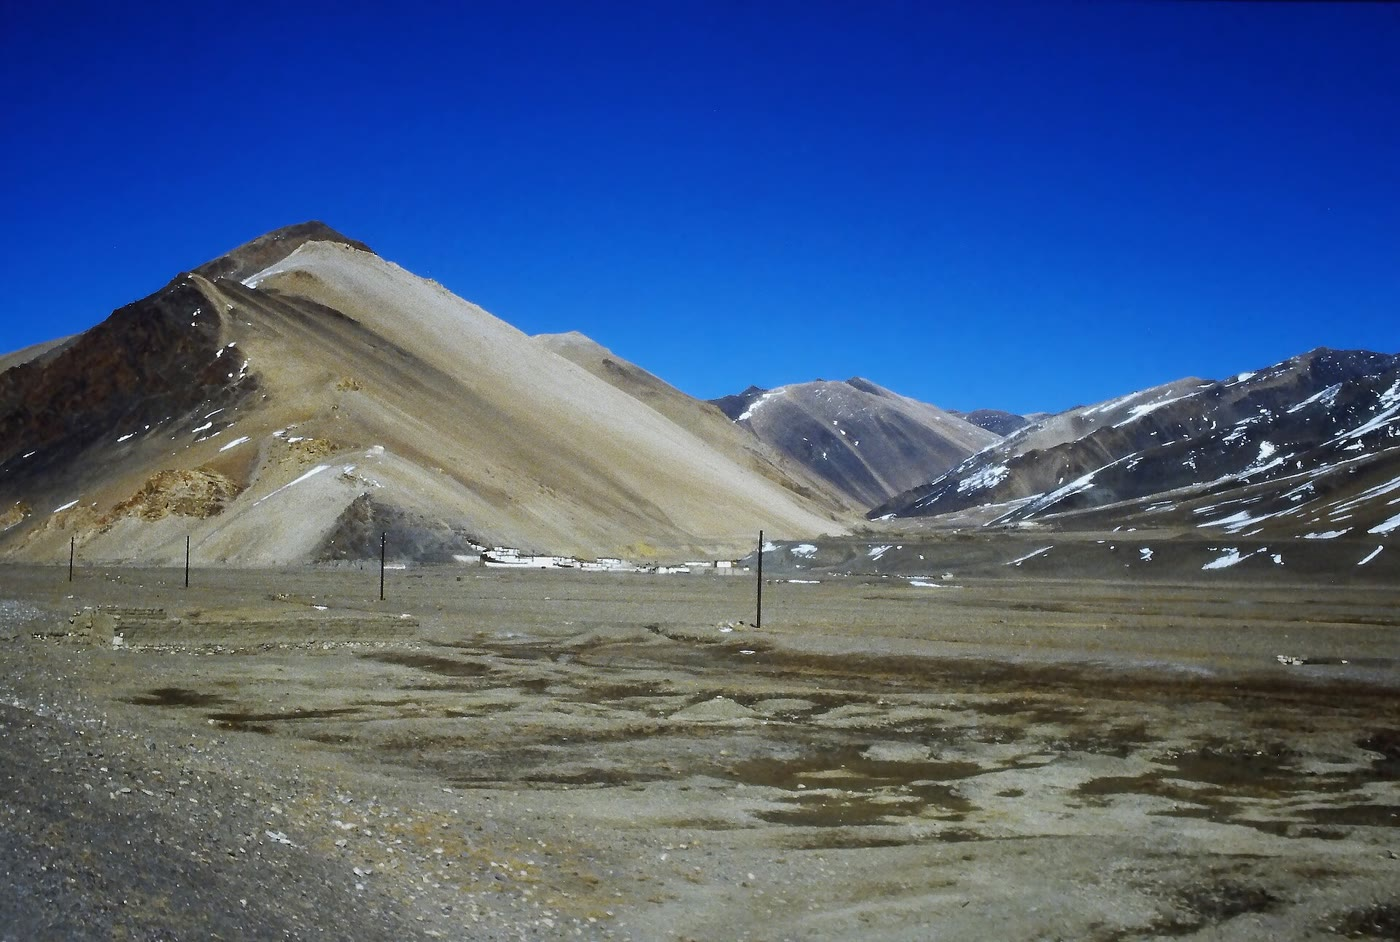
\includegraphics[width=0.66\linewidth]{images/book4/b2-14-tibet-plateau.jpg}
\par\smallskip{\small Dataran Tinggi Tibet di antara Nepal dan Shigatse: dasar datar berupa kerikil dan
padang rumput yang jarang, dengan sebuah desa, di antara pegunungan gundul yang berselimut talus, seluruhnya lebih dari
empat kilometer di atas muka laut.
Foto: Jan Kranendonk, 1987, CC BY-SA 4.0.}
\end{omfigure}
% ledger: data:b4-etopo-tibet

\subsection{Beban sebuah dataran tinggi}

Dataran tinggi membebani sekelilingnya. Pada setiap kedalaman sampai dasar akarnya, sebuah kolom
di bawah dataran tinggi mengalami tekanan lebih tinggi daripada kolom di bawah dataran rendah di sebelahnya;
hanya pada kedalaman kompensasi keduanya sama. Kolom yang tinggi itu mendorong ke luar.

\begin{proposition}[Energi potensial lebih sebuah dataran tinggi]\label{prop:b2:himalaya-andes:gpe}
Di bawah hipotesis \cref{prop:b2:himalaya-andes:airy}, dengan gravitasi $g$, integral
tekanan litostatik lebih kolom dataran tinggi terhadap kolom normal, dari puncak
dataran tinggi sampai kedalaman kompensasi di dasar akarnya $r$, adalah
\[
  \Delta F = \rho_c g h \left(H + \frac{h}{2} + \frac{r}{2}\right) .
\]
Besaran ini adalah energi potensial gravitasi lebih kolom dataran tinggi per satuan luas, dan
gaya per satuan panjang tepi dataran tinggi yang dipakai dataran tinggi itu untuk mendorong
sekelilingnya.
\end{proposition}

\begin{proof}
Ukurlah kedalaman $z$ ke bawah dari muka laut. Dalam kolom dataran tinggi, tekanannya $p_1 =
\rho_c g (z + h)$ dari $z = -h$ sampai $L = H + r$. Dalam kolom normal, tekanannya nol di atas muka
laut, $\rho_c g z$ di dalam kerak, dan $\rho_c g H + \rho_m g (z - H)$ di bawahnya. Selisih $p_1
- p_0$ naik dari 0 pada $z = -h$ sampai $\rho_c g h$ pada muka laut; selisih itu mempertahankan nilai ini di sepanjang
kerak normal, karena di situ kedua kolom sama-sama berupa kerak; di bawah $z = H$ selisih itu berkurang secara linear, sebesar
$(\rho_m - \rho_c) g$ per meter, dan mencapai nol pada $L$ karena $(\rho_m - \rho_c) r = \rho_c
h$. Integralnya adalah luas trapesium ini: $\rho_c g h\,(h/2 + H + r/2)$. Usaha yang dilakukan
tekanan ketika kedua kolom bertukar materi ke samping adalah integral ini, itulah sebabnya integral itu
mengukur baik energi maupun dorongan.
\end{proof}

\begin{omfigure}
\centering
% figdata/bachelor-2/plateaus.py part pressure (h = 4.8 km, H = 35 km, 2700 and 3300 kg/m3)
\begin{tikzpicture}
\begin{axis}[width=0.62\linewidth, height=5.6cm, y dir=reverse, xmin=0, xmax=160, ymin=-12,
  ymax=60, xlabel={tekanan lebih $p_1 - p_0$ (\unit{MPa})}, ylabel={kedalaman di bawah muka laut
  (\unit{km})}, tick label style={font=\scriptsize}, label style={font=\small},
  xtick pos=bottom, ytick pos=left, clip=false]
\addplot[fill=omThm!20, draw=omThm, line width=1pt] table[x expr=\thisrow{p_high_MPa}-\thisrow{p_ref_MPa}, y=z_km] {figdata/out/bachelor-2-plateaus-pressure.dat} \closedcycle;
\draw[dashed] (axis cs:0,0) -- (axis cs:160,0);
\draw[dashed] (axis cs:0,35) -- (axis cs:160,35);
\draw[dashed] (axis cs:0,56.6) -- (axis cs:160,56.6);
\node[font=\scriptsize, anchor=north east] at (axis cs:160,0) {muka laut};
\node[font=\scriptsize, anchor=north east] at (axis cs:160,35) {Moho normal, $H$};
\node[font=\scriptsize, anchor=south east] at (axis cs:160,56.6) {dasar akar, $H + r$};
\node[font=\scriptsize, anchor=west] at (axis cs:100,-8.4) {puncak dataran tinggi, $-h$};
\node[font=\scriptsize, align=center] at (axis cs:60,20) {luas $= \Delta F$\\$\approx\qty{6.1e12}{N.m^{-1}}$};
\end{axis}
\end{tikzpicture}
\par\smallskip{\small Tekanan litostatik lebih kolom dataran tinggi terhadap kolom
normal, untuk $h = \qty{4.8}{km}$, $H = \qty{35}{km}$, dan massa jenis 2700 dan
\qty{3300}{kg.m^{-3}}: tekanan itu naik di sepanjang dataran tinggi, tetap bernilai $\rho_c g h = \qty{127}{MPa}$
di sepanjang kerak normal, dan turun menjadi nol di dasar akar. Daerah berarsir adalah
energi potensial lebih \cref{prop:b2:himalaya-andes:gpe}.}
\end{omfigure}
% values (plateaus.py): tibet_gpe 6.12179e12 N/m for h = 4.8

Untuk Tibet, $r = 4.5 \times 4.8 = \qty{21.6}{km}$ dan $\Delta F = 2700 \times 9.8 \times 4800
\times (35000 + 2400 + 10800) \approx \qty{6.1e12}{N.m^{-1}}$. Bila disebar di atas litosfer
setebal \qty{100}{km}, nilai itu setara dengan tegangan lebih rata-rata sekitar \qty{60}{MPa}, seorde dengan
tegangan yang mematahkan batuan. Dataran tinggi yang seberat itu tidak dapat lagi sekadar naik: dataran tinggi itu cenderung menyebar.

\begin{definition}[Keruntuhan gravitasi]\label{def:b2:himalaya-andes:collapse}
Yang disebut \emph{keruntuhan gravitasi}\index{keruntuhan gravitasi (suatu orogen)} suatu \omterm{def:b2:alpine-orogen:orogen}{orogen}
adalah menyebarnya kerak \omterm{def:b2:alpine-orogen:orogen}{orogen} yang menebal di bawah bebannya sendiri, melalui ekstensi daerah-daerah
tinggi dan aliran atau pensesaran dorong ke luar di tepi-tepinya, yang digerakkan oleh energi potensial lebih
kolom-kolom yang menebal.
\end{definition}

Tibet sedang teregang sementara India masih mendorongnya. Di Tibet selatan, celah-celah berarah utara--selatan
memotong dataran tinggi itu dan mengakomodasi ekstensi timur--barat: seluruhnya sekitar $9 \pm \qty{2}{mm}$ per tahun
antara \ang{81} dan \ang{92}~BT, $1.3 \pm \qty{0.3}{mm}$ per tahun pada celah Yadong--Gulu
saja; di utara Nepal, stasiun GPS menunjukkan dataran tinggi bagian selatan meregang sekitar
\num{12e-9} per tahun. Gempa bumi menceritakan kisah yang sama: pensesaran dorong dan \omterm{def:b2:himalaya-andes:thickening}{penebalan kerak}
mendominasi daerah yang lebih rendah di sekeliling dataran tinggi, sedangkan pensesaran mendatar dan sesar normal mendominasi bagian dalamnya.
Mengapa dataran tinggi itu mengalami ekstensi masih diperdebatkan. Di dataran tinggi bagian timur, ekstensi itu dibaca sebagai \omterm{def:b2:himalaya-andes:collapse}{keruntuhan
gravitasi} yang digerakkan oleh beban dataran tinggi; di selatan, sebagian peneliti mengaitkannya dengan bentuk melengkung
busur Himalaya, yang di sepanjangnya sesar-sesar dorong menyebar, atau dengan India yang menyusup ke bawah.
% ledger: wang21:rifts, ader12:extension

\subsection{Melarikan diri ke samping}

\begin{definition}[Ekstrusi lateral]\label{def:b2:himalaya-andes:extrusion}
Yang disebut \emph{ekstrusi lateral}\index{ekstrusi lateral} (tektonik pelarian) adalah pengusiran
blok-blok kerak atau litosfer ke samping dari zona tumbukan, di sepanjang sesar mendatar besar,
kira-kira tegak lurus arah konvergensi, menuju batas bebas.
\end{definition}

Di timur Tibet, Asia tidak hanya memendek; Asia terdorong ke samping. Sesar-sesar mendatar mengiri
yang panjang, di antaranya sesar Sungai Merah dan sesar Altyn Tagh, dibaca sebagai pemandu
pelarian blok-blok besar ke timur dan tenggara, mula-mula blok Sunda di Asia Tenggara,
lalu Tibet dan Tiongkok Selatan, sementara celah dan cekungan samudra muda membuka di ujung-ujung jauhnya.
Percobaan dengan cetakan kaku yang didorong ke dalam selapis plastisin menghasilkan sesar-sesar semacam itu; model
yang memperlakukan Asia sebagai lembaran kental yang menerus malah menghasilkan penebalan yang luas, tanpa
sesar-sesar besar. GPS mendukung gerakan blok-blok: relatif terhadap Siberia yang stabil, cekungan
Tarim bergerak kira-kira ke utara dengan laju sekitar \qty{14}{mm} per tahun dan Tiongkok Selatan ke arah timur-tenggara
dengan laju sekitar \qty{8}{mm} per tahun. Berapa bagian kemajuan India yang telah diserap oleh penebalan dan berapa
bagian oleh ekstrusi masih diperdebatkan.
% ledger: jiao23:extrusion

\section{Andes}\label{sec:b2:himalaya-andes:andes}

Lempeng Nazca menunjam di bawah Amerika Selatan dengan laju sekitar \qty{72}{mm} per tahun di dekat
\ang{20}~LS, ke arah timur-timur laut, menurut kecepatan sudut NNR-MORVEL56. Tidak ada benua
yang datang, namun Andes Tengah memikul dataran tinggi kedua tertinggi di Bumi.
% ledger: nnr56:poles
% values (plateaus.py): v_nazca_southamerica 72.52 mm/yr, azimuth 74.5

Dari barat ke timur, antara sekitar \ang{15} dan \ang{27}~LS, Andes Tengah terdiri atas lima zona:
\emph{busur muka}; \emph{Cordillera Barat}, yaitu busur vulkanik; dataran tinggi, yaitu
\emph{Altiplano} di utara dan \emph{Puna} di selatan; \emph{Cordillera
Timur}; dan \omterm{def:b2:alpine-orogen:ftb}{sabuk lipatan--sesar dorong} kulit tipis \emph{zona Subandes}, yang
beralih menjadi Dataran Chaco. Profil di atas melintasi zona-zona itu pada \ang{20}~LS: dari parit,
yang simpul terdalamnya terletak \qty{7.7}{km} di bawah muka laut pada \ang{71.4}~BB, permukaan naik
lebih dari \qty{11}{km} dalam jarak sekitar \qty{240}{km} sampai tepi dataran tinggi pada \ang{69.1}~BB;
dataran tinggi itu tetap di atas \qty{3000}{m} sepanjang \qty{440}{km} dengan
rata-rata \qty{3760}{m}. Ketinggian rata-ratanya \qty{3.7}{km} di Altiplano dan \qty{4.4}{km} di
Puna. Di utara \ang{23}~LS, Moho umumnya lebih dalam dari \qty{60}{km}; di bawah
Altiplano tengah, keraknya setebal 59 sampai \qty{64}{km}.
% ledger: gerbault05:andes, gerbault05:moho, data:b4-etopo-andes

\begin{omfigure}
\centering
\begin{tikzpicture}[x=0.56cm, y=0.38cm, font=\scriptsize]
% mantle background
\fill[gray!12] (0,-2.6) -- (5,-3.6) -- (8,-5.6) -- (10,-9.1) -- (12,-12.6) -- (13.2,-14.6) -- (26,-14.6)
  -- (26,-4.5) -- (20,-4.7) -- (17.5,-6.0) -- (15,-7.3) -- (11,-7.0) -- (9.5,-6.2) -- (8,-4) -- (5,-2)
  -- (0,-1) -- cycle;
% ocean water
\fill[blue!8] (0,0) -- (6.33,0) -- (5,-2) -- (0,-1) -- cycle;
% Nazca slab
\fill[gray!45] (0,-1) -- (5,-2) -- (8,-4) -- (10,-7.5) -- (12,-11) -- (14,-14.5) -- (13.2,-14.6)
  -- (12,-12.6) -- (10,-9.1) -- (8,-5.6) -- (5,-3.6) -- (0,-2.6) -- cycle;
% South American crust
\fill[orange!22] (5,-2) -- (8,1) -- (9,1.9) -- (10.2,2.0) -- (11,2.0) -- (15,2.0) -- (15.6,2.6) -- (16.8,2.4)
  -- (17.5,1.6) -- (20,0.6) -- (20.6,0.4) -- (26,0.3) -- (26,-4.5) -- (20,-4.7) -- (17.5,-6.0) -- (15,-7.3)
  -- (11,-7.0) -- (9.5,-6.2) -- (8,-4) -- cycle;
% Altiplano basin fill
\fill[yellow!45] (11,2.0) -- (15,2.0) -- (14.6,1.0) -- (11.4,1.0) -- cycle;
% surface line
\draw[line width=0.5pt] (0,-1) -- (5,-2) -- (8,1) -- (9,1.9) -- (10.2,2.0) -- (11,2.0) -- (15,2.0) -- (15.6,2.6)
  -- (16.8,2.4) -- (17.5,1.6) -- (20,0.6) -- (20.6,0.4) -- (26,0.3);
% arc volcanoes
\fill[red!60!black] (8.8,1.75) -- (9.2,2.9) -- (9.6,1.95) -- cycle;
\fill[red!60!black] (9.8,1.95) -- (10.2,2.8) -- (10.6,2.0) -- cycle;
\draw[red!60!black, decorate, decoration={snake, amplitude=0.6pt, segment length=4pt}] (10.8,-8.0) -- (9.9,1.6);
% Subandean decollement and splays
\draw[thick] (16.0,-1.2) -- (20.55,0.42);
\draw (17.4,-0.7) -- (17.85,1.45);
\draw (18.4,-0.35) -- (18.8,1.08);
\draw (19.4,0.0) -- (19.7,0.72);
% Moho
\draw[dashed] (8,-4) -- (9.5,-6.2) -- (11,-7.0) -- (15,-7.3) -- (17.5,-6.0) -- (20,-4.7) -- (26,-4.5);
% labels
\node at (2.6,-0.5) {Pasifik};
\node at (2.4,-2.2) {lempeng Nazca};
\draw[-{Latex[length=1.6mm]}] (1.6,-2.8) -- (3.2,-3.0);
\node[anchor=south] (tr) at (4.3,0.9) {parit};
\draw[->] (tr.south) -- (5,-1.8);
\node[anchor=south east] at (7.6,1.0) {busur muka};
\node[anchor=south, align=center] at (9.7,3.0) {Cordillera\\Barat (busur)};
\node[anchor=south] at (13,2.1) {Altiplano};
\node[anchor=south, align=center] at (16.4,2.7) {Cordillera\\Timur};
\node[anchor=south west] at (18.6,1.3) {Subandes};
\node[anchor=south] at (23.5,0.4) {Dataran Chaco};
\node at (13,-3.2) {kerak tebal};
\node at (23.2,-2.0) {perisai Brasil};
\node[anchor=north] at (23.2,-4.6) {Moho};
\node at (14.2,-9.6) {baji mantel};
\node at (21,-10) {mantel};
\node[rotate=-50] at (12.75,-12.9) {slab};
\draw[-{Latex[length=2mm]}] (1.2,4.6) -- (0.2,4.6);
\node[anchor=south] at (0.7,4.6) {B};
\draw[-{Latex[length=2mm]}] (24.8,4.6) -- (25.8,4.6);
\node[anchor=south] at (25.3,4.6) {T};
\end{tikzpicture}
\par\smallskip{\small Penampang skematis yang melintasi Andes Tengah di dekat \ang{20}~LS (tidak
berskala). Lempeng Nazca tenggelam di bawah busur muka; \omterm{def:b2:magma-emplacement:magma}{magma} naik dari baji mantel (garis
bergelombang) ke busur Cordillera Barat; Altiplano, dengan isian cekungannya yang tebal, terletak
di antara kedua cordillera, di atas kerak setebal sekitar \qty{60}{km}; sabuk Subandes
kulit tipis tersesar-dorong ke timur di atas perisai Brasil.}
\end{omfigure}
% ledger: gerbault05:andes, gerbault05:moho

\subsection{Bagaimana kerak menjadi tebal}

Dari mana kerak tambahan Altiplano berasal? Kandidat pertama adalah pemendekan:
peraslah sejalur kerak dan jalur itu menebal, dengan mempertahankan luas penampangnya.

\begin{proposition}[Penebalan oleh pemendekan]\label{prop:b2:himalaya-andes:shortening}
Misalkan kerak dengan tebal seragam $H$ memendek, tanpa penambahan atau kehilangan batuan, menjadi kerak
setebal $T$ selebar $W$, dengan penampang tetap sejajar arah pemendekan. Lebar
semulanya $W_0 = W T/H$, dan pemendekannya adalah
\[
  S = W_0 - W = W\,\frac{T - H}{H} .
\]
\end{proposition}

\begin{proof}
Luas penampang kerak itu kekal, seperti pada neraca luas
\cref{prop:b2:alpine-orogen:balance}: $W_0 H = W T$. Karena itu $W_0 = WT/H$ dan $S = W_0 - W =
W(T - H)/H$.
\end{proof}

Pada \ang{20}~LS, dataran tinggi itu selebar sekitar \qty{440}{km}; jika keraknya, yang setebal sekitar \qty{60}{km},
dahulu setebal \qty{35}{km}, pemendekan yang diperlukan adalah $440 \times 25/35 \approx \qty{314}{km}$.
\omterm{def:b2:alpine-orogen:balanced}{Penampang seimbang} di dekat 16--\ang{21}~LS mendapati pemendekan sekitar \qty{50}{km} di Altiplano
dan lebih dari \qty{200}{km} di zona Subandes sejak Oligosen. Volume kerak yang
dihitung dari pemendekan kurang sekitar \qty{20}{\percent} dibandingkan dengan volume yang dihitung dari kedalaman
Moho. Sebagian selisihnya mungkin berasal dari asumsi yang keliru, tentang tebal awal atau
sifat Moho seismik; sebagian mungkin berupa kerak yang ditambahkan dengan cara lain. Satu kompilasi di dekat
\ang{21}~LS menganggap pemendekan tektonik menyumbang sekurang-kurangnya \qty{55}{\percent} akar,
hidrasi baji mantel busur muka sampai \qty{20}{\percent}, dan penambahan magmatik serta
erosi tektonik hanya sekitar \qty{5}{\percent}. Batuan juga dapat berpindah di dalam sabuk:
perbedaan tebal kerak menimbulkan perbedaan energi potensial, seperti di Tibet, dan
perbedaan itu dapat menggerakkan kerak bawah yang panas mengalir dari bagian tebal ke bagian tipis.
% ledger: gerbault05:andes, gerbault05:volume, gerbault05:moho, data:b4-etopo-andes

\begin{omfigure}
\centering
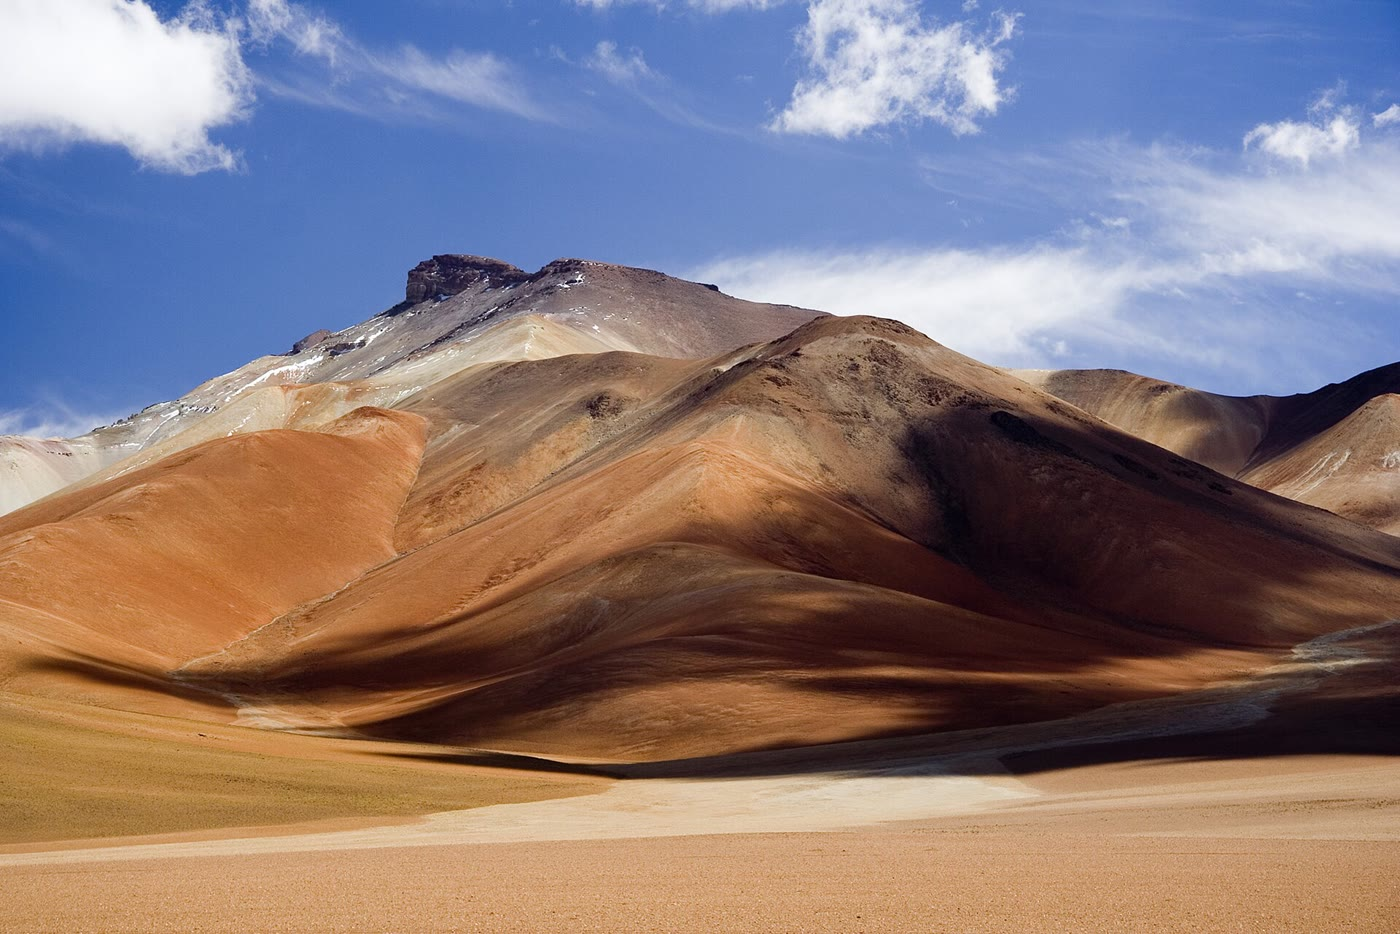
\includegraphics[width=0.66\linewidth]{images/book4/b2-14-altiplano.jpg}
\par\smallskip{\small Altiplano Bolivia: dataran pasir dan kerikil di kaki
perbukitan gundul yang diwarnai merah, oker, dan kelabu oleh batuannya. Foto: Luca Galuzzi, 2006, CC BY-SA 2.5.}
\end{omfigure}
% ledger: gerbault05:andes

\subsection{Slab datar dan akar yang hilang}

Sudut slab tidak tetap, dan sudut itu penting di permukaan.

\begin{definition}[Subduksi slab datar]\label{def:b2:himalaya-andes:flat-slab}
Yang disebut \emph{subduksi slab datar}\index{subduksi slab datar} adalah subduksi yang slabnya,
setelah turun pertama kali, membentang hampir horizontal di bawah lempeng atas sejauh ratusan
kilometer sebelum tenggelam lagi.
\end{definition}

Di sepanjang Andes, dua segmen slab Nazca kini datar, yaitu segmen Peru, yang datar
sejak sekitar \qty{15}{Ma}, dan segmen Pampean, sejak sekitar \qty{18}{Ma}. Di atasnya tidak ada
gunung api aktif. Ketika slab Pampean mendatar, busurnya berpindah ke pedalaman dan meletuskan
lava yang lebih sedikit; di atas segmen-segmen datar itu, busurnya telah diam. Celah busur--parit dari volume Tahun 1
menjelaskan perpindahan ke pedalaman itu: makin landai slab di bawah busur, makin jauh dari parit slab itu
mencapai kedalaman tempat baji meleleh; dan slab yang tetap datar di atas kedalaman itu tidak menyisakan
baji mantel panas yang dapat meleleh sama sekali.
% ledger: gauthier24:flat

\begin{definition}[Delaminasi litosfer]\label{def:b2:himalaya-andes:delamination}
Yang disebut \emph{delaminasi litosfer}\index{delaminasi litosfer} adalah terlepasnya dan
tenggelamnya bagian bawah litosfer yang menebal ke dalam astenosfer, yaitu litosfer mantelnya
dan kadang-kadang kerak bawah yang rapat, yang lalu digantikan oleh astenosfer panas.
\end{definition}

Delaminasi telah diajukan di bawah Puna selatan, antara \ang{24} dan \ang{27}~LS,
sekitar 2 sampai \qty{3}{Ma} yang lalu, tempat lava mafik muda meletus; dan di sepanjang dataran tinggi, perubahan
tebal kerak dan elevasi telah dikaitkan dengan litosfer mantel yang sudah tersingkir
di bawah Altiplano selatan dan belum sepenuhnya tersingkir di bawah Altiplano tengah. Kehilangan
tutup mantel yang rapat membuat kolom yang tersisa lebih ringan: permukaan naik tanpa pemendekan
lagi. Puna sekitar \qty{1}{km} lebih tinggi daripada Altiplano di atas kerak yang sekitar
\qty{11}{km} lebih tipis, suatu kontras yang memerlukan kerak Puna yang lebih ringan atau mantel yang lebih ringan
di bawahnya.
% ledger: gerbault05:delamination, gerbault05:moho

\section{Dua sabuk dibandingkan}\label{sec:b2:himalaya-andes:compared}

Kedua dataran tinggi itu tampak mirip dari jauh dan berbeda dalam hampir segala hal lainnya, seperti yang dihimpun
tabel di bawah.

\begin{omfigure}
\centering\small
\begin{tabular}{>{\raggedright\arraybackslash}p{0.2\linewidth}|>{\raggedright\arraybackslash}p{0.34\linewidth}|>{\raggedright\arraybackslash}p{0.34\linewidth}}
 & Himalaya dan Tibet & Andes Tengah \\ \hline
mesin & benua melawan benua setelah samudra menutup & lempeng samudra yang tenggelam di bawah benua \\
sumbu & sutura dengan \omterm{def:b2:alpine-orogen:ophiolite}{ofiolit} & busur vulkanik di atas slab \\
magmatisme & lelehan kerak: \omterm{def:b2:crustal-melting:leucogranite}{leukogranit} & andesit busur; lava mafik di tempat litosfer hilang \\
konvergensi & sekitar \qty{45}{mm} per tahun, separuhnya diserap di jajaran pegunungan & sekitar \qty{72}{mm} per tahun, sebagian besar habis oleh subduksi \\
gempa bumi besar & pada MHT, Assam 1950, $M_w \approx 8.5$ & pada bidang antarmuka subduksi, Chili 1960, $M_w$ 9.5 \\
dataran tinggi & rata-rata \qty{4.8}{km} sepanjang \qty{1180}{km}; kerak 70--\qty{75}{km} & rata-rata \qty{3.8}{km} sepanjang \qty{440}{km}; kerak sekitar \qty{60}{km} \\
tektonik dataran tinggi & ekstensi timur--barat, ekstrusi & pemendekan di sayap-sayapnya; delaminasi diajukan \\
daratan depan & palung depan Indo-Gangga dan \omterm{def:b2:alpine-orogen:foreland}{molasse} Siwalik & sabuk Subandes dan Dataran Chaco \\
\end{tabular}
\par\smallskip{\small Kedua sabuk berdampingan; sumber-sumbernya dikutip dalam subbab-subbab di atas,
dan gempa bumi Chili adalah yang terbesar yang tercatat sejak 1900.}
\end{omfigure}
% ledger: lave00:setting, lave00:siwaliks, weinberg16:himalaya, ader12:mht, ader12:quakes, usgs:largest, gerbault05:andes, gerbault05:moho, gerbault05:delamination, nnr56:poles, data:b4-etopo-tibet, data:b4-etopo-andes, cattin01:crust, wang21:rifts, jiao23:extrusion

Perbedaan terdalam terletak pada apa yang turun. Di Andes, lempeng samudra terus tenggelam, dan
sebagian besar konvergensi, sekitar \qty{72}{mm} per tahun, habis di parit; pemendekan
lempeng atas sebesar \qty{310}{km} selama sekitar 30 juta tahun hanya akan memakai sekitar \qty{10}{mm} per
tahun darinya. Di Himalaya, tidak ada yang ringan yang dapat tenggelam lama, sehingga konvergensi terpakai untuk
penumpukan, penebalan, dan pendorongan Asia ke samping. Kedua sabuk menumbuhkan dataran tinggi karena kerak yang tebal
adalah kerak yang tinggi; kedua dataran tinggi berhenti naik ketika bebannya sendiri mengimbangi dorongan di
tepinya, lalu menyebar.
% ledger: nnr56:poles, gerbault05:andes, ader12:mht, jiao23:extrusion

\section{Seberapa tinggi gunung dapat menjulang?}\label{sec:b2:himalaya-andes:heights}

Puncak tertinggi, Everest, menjulang \qty{8848.86}{m} di atas muka laut menurut survei bersama
yang diumumkan pada 2020. Mengapa tidak dua puluh kilometer? Batas kasarnya berasal dari kekuatan batuan.

\begin{proposition}[Batas ketinggian dari kekuatan batuan]\label{prop:b2:himalaya-andes:height}
Kolom batuan bermassa jenis $\rho$ yang menjulang setinggi $h$ di atas sekelilingnya, tanpa penopang
lateral di atas aras sekelilingnya, memikul di kakinya tegangan vertikal $\rho g h$ dan
tegangan horizontal nol pada sisi-sisinya yang bebas, sehingga tegangan diferensialnya $\rho g h$. Jika
batuan itu patah pada tegangan diferensial $\sigma_d$, kolom itu hanya dapat berdiri jika $h < \sigma_d/(\rho
g)$.
\end{proposition}

\begin{proof}
Di kaki kolom, tegangan vertikalnya adalah berat batuan di atasnya per satuan luas,
$\rho g h$. Sisi-sisinya bebas, sehingga tegangan horizontal di sana nol. Tegangan
diferensial adalah selisih tegangan utama terbesar dan terkecil, di sini $\rho g h - 0$.
Kepatahan hanya terhindarkan jika tegangan itu tetap di bawah $\sigma_d$.
\end{proof}

Gunung yang sebenarnya memiliki sayap-sayap miring yang menahan intinya, sehingga tegangan di bawahnya
lebih kecil; sebagai orde besaran, ambillah separuhnya, $\rho g h/2$. Untuk Everest, $2700 \times 9.8
\times 8849/2 \approx \qty{117}{MPa}$. Hukum Byerlee dari volume Tahun 1 menempatkan kekuatan gesek
batuan pada sesar di bawah tegangan normal \qty{200}{MPa} pada $50 + 0.6 \times 200 =
\qty{170}{MPa}$: orde yang sama. Gunung yang tiga kali lebih tinggi akan membebani dasarnya jauh melampaui
yang dapat ditanggung batuan; gunung itu akan patah dan menyebar. Di Bumi, puncak setinggi delapan sampai sembilan kilometer
sudah dekat dengan batasnya, dan dataran tinggi, yang menyebar jauh sebelum puncak-puncaknya patah, mendatar
pada ketinggian lima kilometer.
% ledger: tht:everest, byerlee:1975

\section*{Latihan}\label{sec:b2:himalaya-andes:exercises}

Data untuk latihan: $g = \qty{9.8}{m.s^{-2}}$; massa jenis kerak dan mantel
\qty{2700}{kg.m^{-3}} dan \qty{3300}{kg.m^{-3}} kecuali dinyatakan lain; kerak normal $H =
\qty{35}{km}$.

\begin{exercise}[$\star$]\label{exo:b2:himalaya-andes:1}
Sebuah dataran tinggi berada pada elevasi rata-rata \qty{3.0}{km}. Dengan
\cref{prop:b2:himalaya-andes:airy}, hitunglah (a) akar Airy-nya, (b) tebal keraknya.
(c) Seberapa tinggi dataran tinggi itu akan terangkat oleh tambahan kerak \qty{10}{km}?
\end{exercise}

\begin{exercise}[$\star$]\label{exo:b2:himalaya-andes:2}
Sebuah lintasan yang melintasi Himalaya Nepal membentang dari Dataran Gangga ke Dataran Tinggi Tibet.
(a) Sebutkan, berurutan, satuan-satuan yang dilintasinya dan sesar-sesar yang memisahkannya. (b) Sesar mana
yang merupakan sesar normal? (c) Bagaimana derajat \omterm{def:b2:metamorphic-facies:metamorphism}{metamorfisme} berubah ke arah utara sampai Sekuen Himalaya
Besar, lalu di atasnya?
\end{exercise}

\begin{exercise}[$\star$]\label{exo:b2:himalaya-andes:3}
Di Nepal tengah, sebuah teras sungai yang ditinggalkan \qty{9.2}{ka} yang lalu telah memendek sebesar
\qty{196.5}{m} di sepanjang lipatan-lipatan Sesar Dorong Frontal Utama. (a) Hitunglah laju pemendekan
rata-ratanya dalam milimeter per tahun. (b) Bandingkan dengan konvergensi GPS di seluruh jajaran pegunungan,
\qty{17.8}{mm} per tahun. (c) Apa yang dikatakan kesesuaian itu tentang sesar-sesar di utara MFT?
\end{exercise}

\begin{exercise}[$\star$]\label{exo:b2:himalaya-andes:4}
Kelompokkan setiap pengamatan ke dalam \omterm{def:b2:himalaya-andes:types}{orogen tumbukan}, \omterm{def:b2:himalaya-andes:types}{orogen tipe Andes}, atau keduanya: (a) sutura yang dijajari
\omterm{def:b2:alpine-orogen:ophiolite}{ofiolit}; (b) deretan gunung api andesitik aktif; (c) \omterm{def:b2:crustal-melting:leucogranite}{leukogranit} hasil pelelehan
kerak; (d) parit samudra dalam di sepanjang front; (e) \omterm{def:b2:alpine-orogen:foreland}{cekungan depan-pegunungan} dengan \omterm{def:b2:alpine-orogen:foreland}{molasse};
(f) gempa bumi besar pada sesar yang miring landai di bawah jajaran pegunungan.
\end{exercise}

\begin{exercise}[$\star\star$]\label{exo:b2:himalaya-andes:5}
India bergerak \qty{45}{mm} per tahun relatif terhadap Eurasia di Himalaya; di Nepal,
jajaran pegunungan itu sendiri menyerap \qty{17.8}{mm} per tahun di timur dan \qty{20.5}{mm} per tahun di barat.
(a) Berapa fraksi konvergensi yang diserap jajaran pegunungan dalam setiap kasus? (b) Ke mana
sisanya pergi? (c) Selama \qty{10}{Ma}, berapa pemendekan yang diwakili sisanya?
\end{exercise}

\begin{exercise}[$\star\star$]\label{exo:b2:himalaya-andes:6}
(a) Dengan \cref{prop:b2:himalaya-andes:gpe}, hitunglah energi potensial lebih
Altiplano, elevasi rata-rata \qty{3.7}{km}. (b) Bandingkan dengan energi potensial lebih Tibet pada \qty{4.8}{km}.
(c) Tunjukkan bahwa untuk dataran tinggi yang tipis, $h \ll H$, $\Delta F$ tumbuh sebanding dengan $h$, dan untuk
dataran tinggi yang tebal lebih cepat: apa artinya bagi pertumbuhan dataran tinggi?
\end{exercise}

\begin{exercise}[$\star\star$]\label{exo:b2:himalaya-andes:7}
(a) Hitunglah $\rho g h/2$ di bawah Everest, setinggi \qty{8848.86}{m}, dengan $\rho =
\qty{2700}{kg.m^{-3}}$. (b) Menurut hukum Byerlee, $\tau = 0.85\,\sigma_n$ di bawah tegangan normal \qty{200}{MPa}
dan $\tau = \qty{50}{MPa} + 0.6\,\sigma_n$ di atasnya; hitunglah $\tau$ untuk $\sigma_n =
100$ dan \qty{200}{MPa}. (c) Ketinggian berapa yang dimungkinkan oleh kekuatan \qty{170}{MPa}, menurut aturan
orde besaran yang sama?
\end{exercise}

\begin{exercise}[$\star\star$]\label{exo:b2:himalaya-andes:8}
Celah-celah Tibet selatan menyerap ekstensi timur--barat $9 \pm \qty{2}{mm}$ per tahun antara
\ang{81} dan \ang{92}~BT. (a) Berapa lebar bentangan itu pada \ang{30}~LU, dengan \qty{111.19}{km} per
derajat pada meridian? (b) Hitunglah laju regangan ekstensi rata-ratanya, per tahun dan per detik,
beserta rentangnya. (c) Bandingkan dengan $(12.4 \pm 4.7) \times 10^{-9}$ per tahun yang didapat dari GPS di utara Nepal.
\end{exercise}

\begin{exercise}[$\star\star$]\label{exo:b2:himalaya-andes:9}
Sesar Dorong Himalaya Utama yang terkunci di bawah Nepal mengakumulasi defisit momen sebesar
\qty{6.6e19}{N.m} per tahun; gempa-gempa bumi selama 500 tahun terakhir hanya melepaskan
\qty{0.9e19}{N.m} per tahun. (a) Berapa fraksi defisit yang telah dilepaskan? (b) Dengan $M_0 =
10^{1.5 M_w + 9.1}$\,\unit{N.m}, hitunglah momen gempa bumi $M_w$ 8.5. (c) Seberapa sering
gempa bumi semacam itu diperlukan untuk mengimbangi defisit itu?
\end{exercise}

\begin{exercise}[$\star\star\star$]\label{exo:b2:himalaya-andes:10}
Puna \qty{0.7}{km} lebih tinggi daripada Altiplano (4.4 dibandingkan dengan \qty{3.7}{km}) di atas kerak yang
\qty{11}{km} lebih tipis. Ambillah kerak Altiplano setebal \qty{61.5}{km} dan bermassa jenis
\qty{2800}{kg.m^{-3}}, dan mantel \qty{3300}{kg.m^{-3}} di bawah keduanya. (a) Tuliskan
kesamaan massa kedua kolom di atas kedalaman kompensasi bersama. (b) Tentukan
massa jenis yang harus dimiliki kerak Puna jika kerak saja yang mengompensasi perbedaan itu. (c) Bandingkan
dengan 150 sampai \qty{200}{kg.m^{-3}} yang dikutip, dan sebutkan apa lagi yang dapat menjelaskan kontras itu.
\end{exercise}

\begin{exercise}[$\star\star\star$]\label{exo:b2:himalaya-andes:11}
Front vulkanik berada di tempat puncak slab sedalam \qty{105}{km}. (a) Untuk slab yang
miring seragam \ang{30}, hitunglah celah busur--parit dengan rumus dari volume
Tahun 1. (b) Slab itu kini miring \ang{30} sampai kedalaman \qty{90}{km}, lalu hanya \ang{4}: hitunglah
celah yang baru dan pergeseran busur ke pedalaman. (c) Apa yang terjadi pada busur jika slab mendatar
pada kedalaman \qty{95}{km} dan tetap di sana sejauh \qty{300}{km}?
\end{exercise}

\begin{exercise}[$\star\star\star$]\label{exo:b2:himalaya-andes:12}
Erosi menyingkirkan sekitar \qty{300}{km^3} batuan per kilometer Himalaya per juta tahun.
India membawa masuk kerak setebal \qty{37.5}{km} dengan laju \qty{21}{mm} per tahun. (a) Berapa banyak kerak per
kilometer jajaran pegunungan per juta tahun yang masuk ke sabuk itu? (b) Berapa fraksi yang disingkirkan erosi?
(c) Di mana sisanya dapat berada?
\end{exercise}

\begin{problem}[{Soal akhir pekan --- dua dataran tinggi}]\label{pb:b2:himalaya-andes:1}
Profil-profil jalur bab ini memberikan elevasi rata-rata simpul-simpul di Tibet
(\qtyrange{86}{90}{\degree} BT) dan di Andes Tengah (\qtyrange{19}{21}{\degree} LS).
Bila dicuplik setiap \ang{1.5} lintang dan setiap derajat bujur, dan dibulatkan sampai \qty{10}{m}, hasilnya
sebagai berikut. Kecuali dinyatakan lain, $g = \qty{9.8}{m.s^{-2}}$, $\rho_c = \qty{2700}{kg.m^{-3}}$,
$\rho_m = \qty{3300}{kg.m^{-3}}$, dan kerak normal setebal $H = \qty{35}{km}$.

\smallskip
\begin{center}\small
\begin{tabular}{l|ccccccccc}
lintang (\unit{\degree} LU) & 26.5 & 28.0 & 29.5 & 31.0 & 32.5 & 34.0 & 35.5 & 37.0 & 38.5 \\ \hline
elevasi rata-rata (\unit{m}) & 70 & 5000 & 5030 & 4830 & 5020 & 5150 & 5050 & 4470 & 2210
\end{tabular}

\smallskip
\begin{tabular}{l|cccccccc}
bujur (\unit{\degree}) & $-71$ & $-70$ & $-69$ & $-68$ & $-67$ & $-66$ & $-65$ & $-64$ \\ \hline
elevasi rata-rata (\unit{m}) & $-3310$ & 970 & 4150 & 3720 & 3740 & 4010 & 3030 & 1170
\end{tabular}
\end{center}
\smallskip

\noindent\textbf{Bagian I --- Membaca profil.}
\begin{enumerate}
\item Dengan menganggap sampel di atas \qty{3000}{m} sebagai dataran tinggi, hitunglah elevasi rata-rata Tibet
$h_T$, dibulatkan sampai \qty{0.1}{km}.
\item Lakukan hal yang sama untuk Altiplano, $h_A$, dan bandingkan dengan ketinggian rata-rata
\qty{3.7}{km} yang dikutip untuk Altiplano dan \qty{4.4}{km} untuk Puna.
\item Berapa lebar masing-masing dataran tinggi, sekurang-kurangnya, menurut sampel itu (\qty{111.19}{km} per
derajat lintang; \qty{104.5}{km} per derajat bujur pada \ang{20}~LS)?
\item Hitunglah kemiringan rata-rata front Himalaya antara \ang{26.5} dan \ang{28.0}~LU, dalam
persen.
\item Mengapa profil Andes jauh lebih tidak simetris daripada profil Tibet?
\end{enumerate}

\noindent\textbf{Bagian II --- Tebal menurut Airy.}
\begin{enumerate}[resume]
\item Hitunglah akar Airy dan tebal kerak $T_T$ Tibet dari $h_T$.
\item Lakukan hal yang sama untuk Altiplano, $T_A$.
\item Bandingkan dengan tebal seismik, 70 sampai \qty{75}{km} di bawah Tibet dan 59 sampai
\qty{64}{km} di bawah Altiplano tengah. Taksiran mana yang meleset lebih jauh?
\item Massa jenis kerak berapa yang akan membuat tebal Airy untuk Tibet sama dengan \qty{72.5}{km}?
\item Massa jenis berapa yang akan memberikan \qty{61.5}{km} untuk Altiplano?
\item Sebutkan dua alasan, selain massa jenis kerak, mengapa perhitungan Airy lokal dapat
meleset dari akar yang teramati.
\item Kerak setebal \qty{37.5}{km} di bawah India dan \qty{72.5}{km} di bawah Tibet. Dengan
kontras massa jenis di Moho \qty{370}{kg.m^{-3}}, taksirlah dengan lempeng Bouguer, $\Delta g
= 2\pi G\,\Delta\rho\,t$, anomali Bouguer akar Tibet relatif terhadap India, dengan $t$
tebal tambahan di bawah muka laut ($G = \qty{6.674e-11}{m^3.kg^{-1}.s^{-2}}$). Bandingkan dengan
selisih teramati \qty{460}{mGal}.
\end{enumerate}

\noindent\textbf{Bagian III --- Memendekkan Altiplano.} Pada \ang{20}~LS, dataran tinggi itu
selebar \qty{440}{km} dan keraknya setebal sekitar \qty{60}{km}.
\begin{enumerate}[resume]
\item Dengan \cref{prop:b2:himalaya-andes:shortening}, hitunglah lebar pulihan dan
pemendekan yang diperlukan jika kerak itu sebelumnya setebal \qty{35}{km}.
\item \omterm{def:b2:alpine-orogen:balanced}{Penampang seimbang} memberikan pemendekan sekitar \qty{50}{km} di Altiplano dan
\qty{200}{km} di zona Subandes. Berapa fraksi pemendekan yang diperlukan yang hilang?
\item Jika pemendekan hanya membentuk \qty{55}{\percent} kerak tambahan, berapa pemendekan yang
diperlukan?
\item Sabuk Subandes berkulit tipis. Mengapa pemendekannya tetap harus menebalkan kerak
di suatu tempat?
\item Andaikan \qty{314}{km} pada Bagian III terakumulasi selama \qty{30}{Ma}. Hitunglah laju
rata-ratanya, dan fraksi konvergensi Nazca--Amerika Selatan masa kini, \qty{72}{mm} per tahun, yang
diwakilinya.
\item Ke mana sisa konvergensi itu pergi?
\end{enumerate}

\noindent\textbf{Bagian IV --- Beban Tibet.}
\begin{enumerate}[resume]
\item Dengan \cref{prop:b2:himalaya-andes:gpe} dan $h_T$, hitunglah energi potensial lebih Tibet
per satuan luas.
\item Hitunglah energi itu untuk Altiplano dengan $h_A$, serta rasio keduanya.
\item Sebarkan $\Delta F$ Tibet di atas litosfer setebal \qty{100}{km}: tegangan rata-rata berapa yang
diwakilinya?
\item Ekstensi Tibet selatan, \qty{9}{mm} per tahun di sepanjang \qty{1060}{km}, setara dengan regangan berapa
per tahun?
\item Mengapa Tibet dapat mengalami ekstensi timur--barat sementara India masih mendorongnya ke utara?
\item Sebagai ringkasan: berikan tebal kerak Tibet yang dihitung dari elevasi rata-ratanya, dibulatkan
sampai kilometer, dan fraksi \qty{72.5}{km} seismik yang dijelaskannya.
\end{enumerate}
\end{problem}
